\chapter{Integers}
\label{c-int}

\section{Integer numbers}

\begin{description}
    \item [unsigned] All the bits are used for the magnitude of the number. ($0$ to $2^n-1$)
    \item [signed int] The first bit indicates the sign (1 is negative), the remaining $n-1$ bits are used for magnitude. ($-2^{n-1}+1$ to $2^{n-1}-1$)
    \item [1's complement] Positive numbers are the same as signed int, but negative are found by inverting each bit of the positive number with the same magnitude. ($-2^{n-1}+1$ to $2^{n-1}-1$)
    \item [2's complement] As 1's complement, but negative numbers have $1$ added to them after the bitwise inversion.  This removes a $-0$ code, so the extra code is assigned to $-2^{n-1}$.  This is the natural way to handle numbers if addition and subtraction of mixed sign numbers are needed.  ($-2^{n-1}$ to $2^{n-1}-1$)
    \item [$2^{n-1}$ excess] The code is found by adding $2^{n-1}$ to the value (hence the name).  This gives a slightly larger negative range. ($-2^{n-1}$ to $2^{n-1}-1$)
    \item [$2^{n-1}-1$ excess] The code is found by adding $2^{n-1}-1$ to the value (hence the name).  This gives a slightly larger positive range. ($-2^{n-1}+1$ to $2^{n-1}$)
\end{description}

\begin{example}

Convert the following
    \begin{enumerate}
        \item -39 to 8 bit 2's complement

    {\color{ans}
    \begin{tabular}{c|c}
      39 &  \\ \hline
      19 & 1 \\
       9 & 1 \\
       4 & 1 \\
       2 & 0 \\
       1 & 0 \\
       0 & 1 \\
    \end{tabular}

    $39_{10}=100111_2=00100111_2$

    $-39_{10}=11011001_2$
    }
        \item 234 to 8 bit unsigned

    {\color{ans}
    \begin{tabular}{c|c}
      234 &  \\ \hline
      117 & 0 \\
       58 & 1 \\
       29 & 0 \\
       14 & 1 \\
        7 & 0 \\
        3 & 1 \\
        1 & 1 \\
        0 & 1 \\
    \end{tabular}

    $234_{10}=11101010_2$
    }
\end{enumerate}
\end{example}

\section{Addition}

The basic addition routines can be modified to work for any of the codes as well as subtraction for the codes.  The special customizations will be considered later.  Right now, the typical techniques for addition are considered.

\begin{example}
Calculate the following in binary using 8 bits.
    \begin{enumerate}
    \item $42-51$
    \item $51-42$
    \end{enumerate}

    {\color{ans}Sol:

    \begin{tabular}{|c|c|c|}
      \hline
      % after \\: \hline or \cline{col1-col2} \cline{col3-col4} ...
       & 42 & 51 \\
      \hline
      + & 00101010 & 00110011 \\
      - & 11010110 & 11001101 \\
      \hline
    \end{tabular}

    \begin{tabular}{rrrr|rrrr}
      % after \\: \hline or \cline{col1-col2} \cline{col3-col4} ...
       42 &  & 00101010 & &  &  51 &  & 00110011 \\
      -51 &  & 11001101 & &  & -42 &  & 11010110 \\
      \cline{1-1} \cline{3-3} \cline{6-6} \cline{8-8}
         &  &  11110111 & &  &   &  & 100001001 \\
      -9 &  & -00001001 & &  & 9 &  &  00001001 \\
    \end{tabular}
}
\end{example}

\subsection{Ripple Adders}

This is the technique that is covered in CSCI 310.  Basically, full bit adders, see Figure~\ref{f-half_full_add}, are created and cascaded together.  The carry bit from the previous full adder must arrive before the result is added.  The resulting valid carries thus ripple down to the most significant bit (hence the name).  Adding $n$ bit numbers, thus takes the propagation time of $n+1$ levels of logic, i.e. it is O(n) in time to calculate addition.  Thus if 32 bit numbers are added on fast logic (1ns per stage/gate) the process would take 33ns.  This is way too slow.  On the bright side, none of the gates take more than 2 inputs so the size of the gates is O(1).

\begin{figure}
\caption{(left) Half Adder, (right) Full Adder}\label{f-half_full_add}
\begin{center}
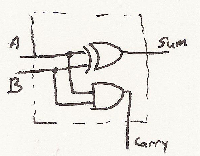
\includegraphics{ha.png} \hspace{.2in} 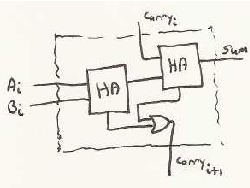
\includegraphics{fa.png}
\end{center}
\end{figure}

\subsection{Conditional Sum}
Conditional sum is a divide and conquer algorithm, and hence exploits binary tree parallelism.  The algorithm works by calculating both possible results for each bit (if carry in was 1 or 0), then performing paired conditional concatenation using the actual carry bit of the lower number, see Figure~\ref{f-cond_sum_add}.

\begin{figure}
\caption{Conditional Sum Adder (above), and its sub-blocks (below, left and right).}\label{f-cond_sum_add}
\begin{center}
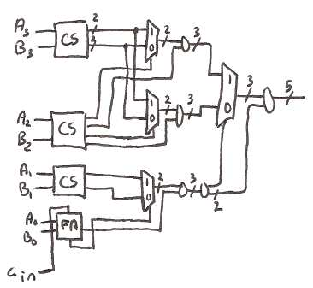
\includegraphics{conditional_sum.png}\\\vspace{.2in}
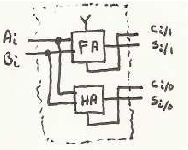
\includegraphics{cs_4out.png} \hspace{.2in} 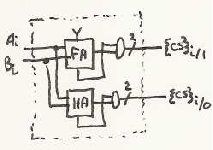
\includegraphics{cs_2out.png}
\end{center}
\end{figure}

\begin{enumerate}
    \item form conditional terms for each digit in summation $\rightarrow$ (digit with carry, digit without carry) = ($x_i+y_i+1$,$x_i+y_i$)
    \item group by twos from right and for both conditional values in the right parenthesis form the result as follows:
    \begin{enumerate}
        \item the leftmost bit of the two terms on the right are the carry bits used to select the term on the left
        \item concatenate the appropriate term on the left (picked by carry) with each term on right after removing the parity bits of the right terms
    \end{enumerate}
    \item continue pairings until only 1 term remains. pick right number if $c_{in}=0$ else pick left.
\end{enumerate}

\begin{example}
 Add $x=0110$ and $y=1111$ by conditional sum and indicate if overflow occurred.

        {\color{ans}
        \begin{tabular}{cccc}
          0+1 & 1+1 & 1+1 & 0+1 \\
          $\downarrow$ & $\downarrow$ & $\downarrow$ & $\downarrow$ \\
          (10,01) & (11,10) & (11,10) & (10,01) \\
          $\searrow$ & $\swarrow$ & $\searrow$ & $\swarrow$ \\
          \multicolumn{2}{r}{(101,100} & \multicolumn{2}{l}{(110,101)} \\
          \multicolumn{2}{c}{$\searrow$} & \multicolumn{2}{c}{$\swarrow$} \\
          \multicolumn{4}{c}{(10110,10101)} \\
          \multicolumn{4}{c}{1 0101} \\
        \end{tabular}

        No overflow occurred (added a positive and negative number).
        }
\end{example}



\begin{example}
    Calculate $7-8$ by conditional sum.

    {\color{ans}

    $7=0111$ and $-8=1000$

    \begin{tabular}{cccc}
    $\;$ 0       & 1          & 1          & 1          \\
      +1         & 0          & 0          & 0          \\ \hline
      (10,01)    & (10,01)    & (10,01)    & (10,01)    \\
      $\searrow$ & $\swarrow$ & $\searrow$ & $\swarrow$ \\
      \multicolumn{2}{c}{(100,011)} & \multicolumn{2}{c}{(100,011)} \\
      \multicolumn{2}{c}{$\quad\searrow$} & \multicolumn{2}{c}{$\swarrow\quad$} \\
      \multicolumn{4}{c}{(10000,01111)} \\
    \end{tabular}

    Since this was done as addition no carry-in was set so the solution is \begin{tabular}{r|l} 0 & 1111 \\ \hline \end{tabular} or $-1$ in signed base ten.

    }
\end{example}


\begin{example}
Add by conditional sum $x=01100110$ and $y=00110011$.

{\color{ans}
\noindent
\begin{tabular}{rrrrrrrr}
$0+0$ & $1+0$ & $1+1$ & $0+1$ & $0+0$ & $1+0$ & $1+1$ & $0+1$ \\
$\downarrow$ & $\downarrow$ & $\downarrow$ & $\downarrow$ & $\downarrow$ & $\downarrow$ & $\downarrow$ & $\downarrow$ \\
$(01,00)$ & $(10,01)$ & $(11,10)$ & $(10,01)$ & $(01,00)$ & $(10,01)$ & $(11,10)$ & $(10,01)$ \\
$\searrow$ & $\downarrow$ & $\searrow$ & $\downarrow$ & $\searrow$ & $\downarrow$ & $\searrow$ & $\downarrow$ \\
\multicolumn{2}{r}{$(010,001)$} & \multicolumn{2}{r}{$(110,101)$} & \multicolumn{2}{r}{$(010,001)$} & \multicolumn{2}{r}{$(110,101)$} \\
& $\searrow$ & & $\swarrow$ & & $\searrow$ & & $\swarrow$  \\
&  & \multicolumn{2}{c}{$(01010,01001)$} &  &  & \multicolumn{2}{c}{$(01010,01001)$ }  \\
&  &  & $\searrow$ &  & $\swarrow$ &  &  \\
&  &  & \multicolumn{3}{c}{$(010011010,010011001)$} &  &  \\
&  &  & \multicolumn{3}{c}{$0 \, 10011001$} &  &  \\
\end{tabular}
}
\end{example}

Why go through this?  First, by a folk theorem of Dr. Alan Laub, ``\emph{What is hard for us tends to be easy for computers (and vice versa)}.''  In reality this process is really easy for a computer to do.  Second, the process is highly parallel, so it can be done very fast.  If the numbers to be added are n bits long this takes $2(\log_2(n)+1)$ levels of logic, much better than the $n+1$ levels of logic required by ripple calculations.  Thus it is O(log(n)) in time complexity.  For example, for adding the 32 bit numbers considered already, conditional sum would take $2(\log_2(32)+1)=12$ levels of logic, so on the fast logic described it would be 12ns, a huge improvement.

\subsection{Carry-Lookahead}

This is also referred to as lookahead carry.  Assume $x+y=z$.  Pre-generate all carries with 2-level logic. Usually form (g,p,c) generate, propagate, carry.
\beqn
G_i & = & x_i \cdot y_i \\
P_i & = & x_i + y_i \\
C_i & = & G_i + P_i \cdot C_{i-1} \\
    & = & G_i + P_i \cdot (G_{i-1} + P_{i-1} \cdot C_{i-2}) \\
    & = & G_i + P_i \cdot G_{i-1} + P_i \cdot P_{i-1} \cdot C_{i-2} \\
    & = & G_i + P_i \cdot G_{i-1} + P_i \cdot P_{i-1} \cdot G_{i-2} +
    \ldots + P_i \cdot P_{i-1} \cdot \ldots \cdot P_0 \cdot C_{in}
\eeqn

This method is very fast (regardless of size it take 5 levels of logic) but requires large gates for problems of reasonable size (even 16 or 32 bit numbers) and thus has problems with fan-in, fan-out, and size.

Often blocks of a number are handled with lookahead, and the blocks are connected in some fashion (for example ripple) to get the net result (i.e. just like single bit adds from a full adder are connected to propagate the carry bit, blocks or 4, 8, or more could be handled lookahead then connected to propagate the carry bit between them to handle a larger number, say 32 bits).  Even better than cascading (ripple connection) the adders, is to us group carry-lookahead, in which each of the carry-lookahead adders output their group propagate and group generate variables to a circuit that generates the carry-in bits for each group.  It takes 5 logic levels to generate the carries to each individual carry-lookahead adder, and each adder then takes 5 levels of logic to get the result, for a total of 10 levels of logic.  For the example of adding 32 bit numbers with fast logic, it would take 10ns with group carry-lookahead adders (probably four or eight bits in a group).


\begin{example}
Specify the equations of a two bit binary adder with carry in (i.e.: one equation for each of the sum bits and one equation for the carry out).  Put the equations in sum of products form.

{\color{ans}Sol:
Let the two numbers to be added be $A_1 A_0$ and $B_1 B_0$.  Let the resulting sum be $S_1 S_0$.  Let the carries be $C_{in}$ and $C_{out}$.  Finally, let $C_0$ be the carry from the first bit added (saves writing).
\beqn
S_0 & = & A_0 \oplus B_0 \oplus C_{in} \\
C_0 & = & A_0\cdot B_0 + A_0\cdot C_{in} + B_0\cdot C_{in} \\
S_1 & = & A_1 \oplus B_1 \oplus C_0\\
C_{out} & = & A_1 \cdot B_1 + A_1 \cdot C_0 + B_1 \cdot C_0
\eeqn
Putting this in sum of products form yields
\beqn
S_0 & = & A_0' \cdot B_0' \cdot C_{in} +
          A_0' \cdot B_0 \cdot C_{in}' +
          A_0 \cdot B_0' \cdot C_{in}' +
          A_0 \cdot B_0 \cdot C_{in} \\
S_1 & = & A_1' \cdot B_1' \cdot (A_0\cdot B_0 + A_0\cdot C_{in} + B_0\cdot C_{in}) +
          A_1' \cdot B_1 \cdot (A_0\cdot B_0 + A_0\cdot C_{in} + B_0\cdot C_{in})' + \\
    & & \qquad A_1 \cdot B_1' \cdot (A_0\cdot B_0 + A_0\cdot C_{in} + B_0\cdot C_{in})' +
          A_1 \cdot B_1 \cdot (A_0\cdot B_0 + A_0\cdot C_{in} + B_0\cdot C_{in}) \\
    & = & A_1' \cdot B_1' \cdot A_0\cdot B_0 + A_1' \cdot B_1' \cdot A_0 \cdot C_{in}
          + A_1' \cdot B_1' \cdot B_0\cdot C_{in} \\
    & & \qquad
          + A_1' \cdot B_1 \cdot (A_0'\cdot B_0' + A_0'\cdot C_{in}' + B_0'\cdot C_{in}') \\
    & & \qquad
          + A_1 \cdot B_1' \cdot (A_0'\cdot B_0' + A_0'\cdot C_{in}' + B_0'\cdot C_{in}') \\
    & & \qquad
          + A_1 \cdot B_1 \cdot A_0\cdot B_0 + A_1 \cdot B_1 \cdot A_0\cdot C_{in}
           + A_1 \cdot B_1 \cdot B_0\cdot C_{in} \\
    & = & A_1' \cdot B_1' \cdot A_0\cdot B_0 + A_1' \cdot B_1' \cdot A_0 \cdot C_{in}
          + A_1' \cdot B_1' \cdot B_0\cdot C_{in} \\
    & & \qquad
          + A_1' \cdot B_1 \cdot A_0'\cdot B_0' + A_1' \cdot B_1 \cdot A_0'\cdot C_{in}'
          + A_1' \cdot B_1 \cdot B_0'\cdot C_{in}' \\
    & & \qquad
          + A_1 \cdot B_1' \cdot A_0'\cdot B_0' + A_1 \cdot B_1' \cdot A_0'\cdot C_{in}'
          + A_1 \cdot B_1' \cdot B_0'\cdot C_{in}' \\
    & & \qquad
          + A_1 \cdot B_1 \cdot A_0\cdot B_0 + A_1 \cdot B_1 \cdot A_0\cdot C_{in}
           + A_1 \cdot B_1 \cdot B_0\cdot C_{in} \\
C_{out} & = & A_1 \cdot B_1 + A_1 \cdot (A_0\cdot B_0 + A_0\cdot C_{in} + B_0\cdot C_{in}) \\
   & & \qquad + B_1 \cdot (A_0\cdot B_0 + A_0\cdot C_{in} + B_0\cdot C_{in}) \\
    & = & A_1 \cdot B_1 + A_1 \cdot A_0\cdot B_0 + A_1 \cdot A_0\cdot C_{in} + A_1 \cdot B_0\cdot C_{in} \\
   & & \qquad + B_1 \cdot A_0\cdot B_0 + B_1 \cdot A_0\cdot C_{in} + B_1 \cdot B_0\cdot C_{in}
\eeqn
}
\end{example}

\subsection{Other notes}

Integer numbers larger than the word size of the computer can be handled by chaining.  Two special assembly commands are often available to aid in chaining: addc, subb.   Normally when you add the first carry in is zero, but for blocks of bits after the first block, the lower block might need to carry up.  Addc uses the carry bit as $c_{in}$ rather than assuming $c_{in}=0$.

Two different signals are used to warn that the integer result might not be valid\footnote{Overflow and carry are two of the typical condition codes.  It is possible for a condition code to be set but the result is still valid.  For instance carry could be set and overflow could be unset after an operation with 2's complement numbers.  In this case the number is still valid since overflow is the signal for 2's complement.} : carry (c) and overflow (v).  Carry is used for unsigned integers, and overflow is used for two's complement.  Since both carry and overflow bits are both calculated at the same time\footnote{On some machines every arithmetic operation generates the condition codes, on other machines, like the SPARC, the condition codes are set only when special versions of the arithmetic commands that end in \emph{cc} are used.} it is important to know what they mean, when they are relevant, and how they are calculated.

Overflow set if last two carries are different.



\subsection{Signed Int}

Addition
\begin{itemize}
    \item if signs are same then add two $n-1$ digit numbers and keep sign
    \item else flip sign of second term and subtract (subtracting with same signs).
\end{itemize}

\noindent
Subtraction ($S_1-S_2$)
\begin{itemize}
    \item if $S_1 \ge S_2 \ge 0$ or $S_1 \le S_2 < 0$ then preserve sign and subtract absolute magnitudes,
    \item if $S_2 > S_1 \ge 0$ or $S_2 < S_1 < 0$ then flip sign and subtract absolute magnitudes reversed,
    \item else flip sign of second term and add (adding with same signs).
\end{itemize}

\subsection{2's Comp}

For addition you just add the numbers normally with $c_{in}=0$(no special cases).

For subtraction you take the 1's complement of the second number and add with $c_{in}=1$(no special cases, note 1's complement +1 is 2's complement).

\subsection{Excess}

For addition, you need to carry extra bits while calculating, because you have to subtract the excess number after adding.  This is needed because the excess was in each of the numbers added, so an extra excess is present which must be removed.

For subtraction, the excess gets removed in the process so it must be added back in after subtraction.  Note the subtraction can result in an intermediate negative number, so extra bits are needed during calculation.

\section{Multiplication}

\subsection{unsigned}

Algorithm 1
\begin{enumerate}
    \item set \emph{v} to 0
    \item for each digit do:
    \begin{enumerate}
        \item if lsb of \emph{x} is 1, add \emph{y} to \emph{v}
        \item left shift \emph{y}
        \item right shift \emph{x}
    \end{enumerate}
\end{enumerate}

This basically only handles numbers whose product fits in 1 register.  In general multiplication could take up to 2 registers.

\noindent
Algorithm 2
\begin{enumerate}
    \item group two regs (\emph{u},\emph{v}) for product, set to 0
    \item for each digit do:
    \begin{enumerate}
        \item  add (\emph{y} and lsb(x)) to \emph{u} hold carry in \emph{c}
        \item right shift (\emph{c},\emph{u},\emph{v})
        \item circulant right shift \emph{x}
    \end{enumerate}
\end{enumerate}

Right shifting the product with carry is the same as left shifting (\emph{$y_{hi}$},\emph{y}), but without the need for a second register to hold the high order bits.  The algorithm can be implemented in a circuit as is done in Figure~\ref{f-unsigned_mult}.

\begin{figure}
\caption{Unsigned Multiplier of Algorithm 2}\label{f-unsigned_mult}
\begin{center}
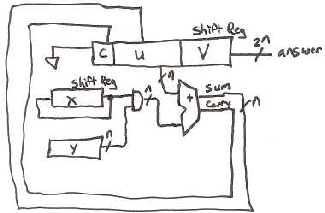
\includegraphics{unsigned_mult.png}
\end{center}
\end{figure}

\begin{example}
Multiply 10 and 12 in binary using algorithm 2

{\color{ans}
First we need to convert our numbers to binary: $x=10_{10} = 1010_2$ and $y=12_{10} = 1100_2$.

\begin{tabular}{ccccp{2in}}
c & u    & v    & x    & Comments  \\\hline
0 & 0000 & 0000 & 1010 & Setup (Step 1) \\\hline
  &      &      &      & Round 1\\
0 & 0000 &      &      & Step 2a: add $y\cdot 0$ to u (0+0=0)\\
0 & 0000 & 0000 &      & Step 2b: rotate right cuv \\
  &      &      & 0101 & Step 2c: circulant right shift x \\
0 & 0000 & 0000 & 0101 & End of round 1 \\\hline
  &      &      &      & Round 2\\
0 & 1100 &      &      & Step 2a: add $y\cdot 1$ to u (0+12=12)\\
0 & 0110 & 0000 &      & Step 2b: rotate right cuv \\
  &      &      & 1010 & Step 2c: circulant right shift x \\
0 & 0110 & 0000 & 1010 & End of round 2 \\\hline
  &      &      &      & Round 3\\
0 & 0110 &      &      & Step 2a: add $y\cdot 0$ to u (6+0=6)\\
0 & 0011 & 0000 &      & Step 2b: rotate right cuv \\
  &      &      & 0101 & Step 2c: circulant right shift x \\
0 & 0011 & 0000 & 0101 & End of round 3 \\\hline
  &      &      &      & Round 4\\
0 & 1111 &      &      & Step 2a: add $y\cdot 1$ to u (3+12=15)\\
0 & 0111 & 1000 &      & Step 2b: rotate right cuv \\
  &      &      & 1010 & Step 2c: circulant right shift x \\
0 & 0111 & 1000 & 1010 & End of round 4 \\\hline
\end{tabular}

Note $x$ is returned to its original value and $uv = 01111000_2 = 120_{10}$.
}
\end{example}

\begin{example}
Multiply 14 and 7 in binary using algorithm 2

{\color{ans}
First we need to convert our numbers to binary: $x=14_{10} = 1110_2$ and $y=7_{10} = 0111_2$.

\begin{tabular}{ccccp{2in}}
c & u    & v    & x    & Comments  \\\hline
0 & 0000 & 0000 & 1110 & Setup (Step 1) \\\hline
  &      &      &      & Round 1\\
0 & 0000 &      &      & Step 2a: add $y\cdot 0$ to u (0+0=0) \\
0 & 0000 & 0000 &      & Step 2b: rotate right cuv \\
  &      &      & 0111 & Step 2c: circulant right shift x \\
0 & 0000 & 0000 & 0111 & End of round 1 \\\hline
  &      &      &      & Round 2\\
0 & 0111 &      &      & Step 2a: add $y\cdot 1$ to u (0+7=7) \\
0 & 0011 & 1000 &      & Step 2b: rotate right cuv \\
  &      &      & 1011 & Step 2c: circulant right shift x \\
0 & 0011 & 1000 & 1011 & End of round 2 \\\hline
  &      &      &      & Round 3\\
0 & 1010 &      &      & Step 2a: add $y\cdot 1$ to u (3+7=10) \\
0 & 0101 & 0100 &      & Step 2b: rotate right cuv \\
  &      &      & 1101 & Step 2c: circulant right shift x \\
0 & 0101 & 0100 & 1101 & End of round 3 \\\hline
  &      &      &      & Round 4\\
0 & 1100 &      &      & Step 2a: add $y\cdot 1$ to u (5+7=12) \\
0 & 0110 & 0010 &      & Step 2b: rotate right cuv \\
  &      &      & 1110 & Step 2c: circulant right shift x \\
0 & 0110 & 0010 & 1110 & End of round 4 \\\hline
\end{tabular}

Note $x$ is returned to its original value and $uv = 01100100_2 = 98_{10}$.
}
\end{example}

\subsection{2's complement}

Human's have tons of shortcuts to speed up our calculations, so it should come as no surprise that it is similar with digital circuits.  One shortcut we often use in calculating things is based on estimating.  Say you wanted to multiply $99$ and $56$.  It would be easier to do it as $(100-1)*56=5600-56=5544$.  It would be no different if we wanted to multiply $99,099$ and $56$; just do $f(100,000-1,000+100-1)*56=5,600,000-56,000+5,600-56=5,549,544$.  This technique forms the basis of Booth's Algorithm, which works even nicer since we are dealing with binary.  Consider, $0111_2$ times $011_2$.  The first number can be written as $01000_2 - 01_2$, so we have $(01000_2-01_2)*011_2=011000_2-011_2=010101_2$.  We want to find a pattern to do this automatically, so lets consider a slightly bigger example: $01100111_2 * 011_2$ or $103* 3$.  We need to break up the first number, and we will add a radix point and do it in a table to make it easier to see something:

\begin{tabular}{ccccccccc@{ . }c}
0 & 0 & 1 & 1 & 0 & 0 & 1 & 1 & 1 & 0\\ \hline
0 & 1 & 0 & 0 & 0 & 0 & 0 & 0 & 0 & 0\\
- & 0 & 0 & 1 & 0 & 0 & 0 & 0 & 0 & 0\\
+ & 0 & 0 & 0 & 0 & 1 & 0 & 0 & 0 & 0\\
- & 0 & 0 & 0 & 0 & 0 & 0 & 0 & 1 & 0\\
\end{tabular}

Notice that in the original number when the current digit is a zero and the previous was a 1 we add a 1 (I will highlight this in blue), and when the current digit is a 1 and the previous was a 0 we subtract 1 (I will highlight this in red):

\begin{tabular}{ccccccccc@{ . }c}
0 & {\color{blue}0}
      & {\color{blue}1}
          & {\color{red}1}
              & {\color{red}0}
                  & {\color{blue}0}
                      & {\color{blue}1}
                          & 1 & {\color{red}1}
                                  & {\color{red}0}\\ \hline
0 & {\color{blue}1}
      & 0 & 0 & 0 & 0 & 0 & 0 & 0 & 0\\
- & 0 & 0 & {\color{red}1}
              & 0 & 0 & 0 & 0 & 0 & 0\\
+ & 0 & 0 & 0 & 0 & {\color{blue}1}
                      & 0 & 0 & 0 & 0\\
- & 0 & 0 & 0 & 0 & 0 & 0 & 0 & {\color{red}1}
                                  & 0\\
\end{tabular}

I like this pattern, because $10_2$ is a negative number in two's compliment and that is where I subtract, and $01_2$ is a positive number in two's compliment and that is where I add.  It is thus memorable.  Since we are multiplying the location of the 1's tell us where to add or subtract the other number.  Thus we have in our example (with one extra column to fit the multiplied numbers):

\begin{tabular}{cccccccccc@{ . }c}
0 & {\color{blue}1}
      & {\color{blue}1}
          & 0 & 0 & 0 & 0 & 0 & 0 & 0 & 0\\
- & 0 & 0 & {\color{red}1}
              & {\color{red}1}
                  & 0 & 0 & 0 & 0 & 0 & 0\\
+ & 0 & 0 & 0 & 0 & {\color{blue}1}
                      & {\color{blue}1}
                          & 0 & 0 & 0 & 0\\
- & 0 & 0 & 0 & 0 & 0 & 0 & 0 & {\color{red}1}
                                  & {\color{red}1}
                                      & 0\\\hline
0 & 1 & 0 & 0 & 1 & 1 & 0 & 1 & 0 & 1 & 0\\
\end{tabular}

So we find that $01100111_2 * 011_2=0100110101_2$ or $103*3=309$.  It is worth noting a couple things in the resulting pattern. First, since we alternate addition and subtraction it is impossible to get overflow, and thus the carry bit isn't needed.  Second, if we were multiplying by a negative number, like $-2_{10}=10_2=110_2=1110_2$, we can note the leftmost of our $01$ or $10$ patterns is $10$, which means subtract.  The leftmost is the most significant, thus a negative number times a positive number would result in a negative.  If you think about it a negative times a negative will result in a positive.  This means our technique handles signed multiplication directly! Since this works nicely we want to generalize it, which is what we have as Booth's algorithm.

\textbf{Booth's Algorithm}
\begin{enumerate}
    \item group two regs (\emph{u},\emph{v}) for product, set to 0
    \item set \emph{$x_{-1}$} to 0 (this is a single bit)
    \item for each digit do:
    \begin{enumerate}
        \item if (lsb of \emph{x} is 1,) and (\emph{$x_{-1}$}=0), subtract \emph{y} from \emph{u}
        \item if (lsb of \emph{x} is 0) and (\emph{$x_{-1}$}=1), add \emph{y} to \emph{u}
        \item arithmetic right shift (\emph{u},\emph{v})
        \item circular right shift \emph{x}
    \end{enumerate}
\end{enumerate}

Booth's algorithm can be implemented in a circuit as is done in Figure~\ref{f-booths}.

\begin{figure}
\caption{Booth's Algorithm}\label{f-booths}
\begin{center}
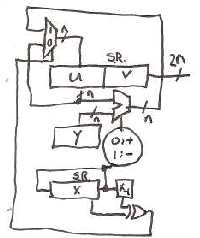
\includegraphics{booths.png}
\end{center}
\end{figure}


\begin{example}
Multiply $6$ ($x=0110$) and $-1$ ($y=1111$) using Booth's algorithm.  Show the values at each stage in a table.

       {\color{ans}
       Booth's

       \begin{tabular}{cccc}
         $u$ & $v$ & $x$ & $x_{-1}$ \\ \hline
         0000 & 0000 & 1111 & 0 \\ \hline
         1010 & 0000 &   &   \\
         1101 & 0000 & 1111 & 1 \\ \hline
         1110 & 1000 & 1111 & 1 \\ \hline
         1111 & 0100 & 1111 & 1 \\ \hline
         1111 & 1010 & 1111 & 1 \\
       \end{tabular}

       Note the answer is 11111010, which is $-6$ in 2's complement.
       }
\end{example}

\begin{example}
Multiply -3 and 5 using Booth's algorithm and 4 bit numbers.  Perform the indicated calculations showing all steps.

    {\color{ans}
    $y=5=0101$

    $-y=-5=1011$

    \begin{tabular}{|c|c|cc|} \hline
      $u$  & $v$  & $x$  & $x_{-1}$ \\ \hline
      0000 & 0000 & 1101 & 0 \\ \hline
      1011 &      &      &   \\ \cline{1-1}
      1011 & 0000 & 1101 & 0 \\
      1101 & 1000 & 1110 & 1 \\ \hline
      0101 &      &      &   \\ \cline{1-1}
      0010 & 1000 & 1110 & 1 \\
      0001 & 0100 & 0111 & 0 \\ \hline
      1011 &      &      &   \\ \cline{1-1}
      1100 & 0100 & 0111 & 0 \\
      1110 & 0010 & 1011 & 1 \\ \hline
      1111 & 0001 & 1101 & 1 \\ \hline
    \end{tabular}

    The result is 11110001, which is $-15$ in 2's complement.
    }
\end{example}

\begin{example}
Multiply -3 and -6 using Booth's algorithm and 4 bit numbers.  Perform the indicated calculations showing all steps.

    {\color{ans}

    $x=-3=1101$, $y=-6=1010$ and $-y=6=0110$.

    \begin{tabular}{|c|c|c|c|}
      \hline
      $U$ & $V$ & $X$ & $X_{-1}$ \\ \hline
      0000 & 0000 & 1101 & 0 \\ \hline
      0110 & 0000 & 1101 & 0 \\
      0011 & 0000 & 1110 & 1 \\ \hline
      1101 & 0000 & 1110 & 1 \\
      1110 & 1000 & 0111 & 0 \\ \hline
      0100 & 1000 & 0111 & 0 \\
      0010 & 0100 & 1011 & 1 \\ \hline
      0001 & 0010 & 1101 & 1 \\ \hline
    \end{tabular}

    $00010010=18$
    }
\end{example}

\subsection{Systolic Array}

The preceding algorithms are $O(n^2)$ if implemented with ripple adders, $O(n\log(n))$ if implemented with conditional sum adders, or $O(n)$ if implemented with look-ahead adders.  The look-ahead adders have a large constant, so the $O(n)$ is not a perfect indicator of performance, and they are currently not practical beyond about 8 bits.  It would be nice to find a way to multiply that has $O(n)$ and a small constant multiplier.  Systolic arrays are $O(n)$, and have a constant multiplier of about 6 depending on your hardware, which is about half what it takes with even block (group) carry look-ahead adders using serial routines.

\begin{figure}[p]
  \SystolicCell
  \caption{Individual Cell of Systolic Array}\label{fig-systolic-cell}
\end{figure}

\begin{figure}[p]
  \SystolicArray
  \caption{Systolic Array For 4 Bit Numbers}\label{fig-systolic-array}
\end{figure}


\section{Integrated Examples}







\begin{example}
Calculate the following expression in binary using 2's
complement and 8 bits total.  Show all work.
\beqn
(9*9-24)/3
\eeqn
{\color{ans}
Sol:

$9_{10}=00001001_{2}$ and $3_{10}=00000011_{2}$

\begin{tabular}{l|l}
24 & \\
\hline
12 & 0 \\
6 & 0 \\
3 & 0 \\
1 & 1 \\
0 & 1 \\
\end{tabular}

$24_{10}=00011000_{2}$ thus $-24_{10}=11101000_{2}$.
Thus $9*9$,

\begin{tabular}{cccccccccccc}
&&&&0&0&0&0&1&0&0&1 \\
&&&&0&0&0&0&1&0&0&1 \\
\hline
&&&&0&0&0&0&1&0&0&1 \\
&0&0&0&0&1&0&0&1&&& \\
\hline
&&&&0&1&0&1&0&0&0&1 \\
\end{tabular}

Then (subtracting 24),

\begin{tabular}{ccccccccc}
&0&1&0&1&0&0&0&1 \\
&1&1&1&0&1&0&0&0 \\
\hline
1&0&0&1&1&1&0&0&1 \\
&0&0&1&1&1&0&0&1 \\
\end{tabular}

Now perform the division:

\begin{tabular}{cccccccc}
&&&1&0&0&1&1 \\ \cline{3-8}
1 & 1 & \multicolumn{1}{|c}{1} & 1 & 1 & 0 & 0 & 1 \\
  &   & 1 & 1 &   &   &   & \\ \cline{3-4}
  &   &   & 0 & 1 & 0 & 0 & \\
  &   &   &   &   & 1 & 1 & \\ \cline{6-7}
  &   &   &   &   &   & 1 & 1 \\
  &   &   &   &   &   & 1 & 1 \\ \cline{7-8}
  &   &   &   &   &   &   & 0 \\
\end{tabular}

The answer is thus $00010011_{2} = 19_{10}$.
}
\end{example}



\section{Residue Arithmetic}

We have shown different ways of calculating the sum and product of binary numbers.  In this section we will examine a different way to represent numbers and thus to calculate.  In residue arithmetic numbers are represented by their remainders of a group of numbers that constitute the basis of the representation.   Let's consider a simple example of how numbers can be represented in this method.

\begin{tabular}{|l|cc|} \hline
  Number & \%2 & \%3 \\ \hline
  0      & 0   & 0   \\
  1      & 1   & 1   \\ \hline
  2      & 0   & 2   \\
  3      & 1   & 0   \\ \hline
  4      & 0   & 1   \\
  5      & 1   & 2   \\ \hline
\end{tabular}

Note that each of the numbers from 0 through 5 can be represented uniquely by their remainders.  Note that the number 6 would be 0,0 and thus not distinguishable from 0.  You can represent six numbers (1-5) because the product of the basis numbers is $2\times 3=6$.  That we can represent the numbers is one thing, being able to calculate easily is another.  Lets consider addition first:

\begin{tabular}{r@{=}lcr@{=}l}
1 & 1,1               && 2 & 0,2 \\
2 & 0,2               && 3 & 1,0 \\ \cline{1-2}\cline{4-5}
3 & (0+1)\%2,(1+2)\%3 && 5 & (0+1)\%2,(2+0)\%3 \\
  & 1,0               &&   & 1,2 \\
\end{tabular}

If you look up (1,0) in our table you will find it corresponds to 3, similarly (1,2) corresponds to 5.  Now lets try some multiplication problems:

\begin{tabular}{r@{=}lcr@{=}l}
2 & 0,2                               && 1 & 1,1 \\
2 & 0,2                               && 3 & 1,0 \\ \cline{1-2}\cline{4-5}
4 & ($0\times 0$)\%2,($2\times 2$)\%3 && 3 & ($1\times 1$)\%2,($1\times 0$)\%3 \\
  & 0,1                               &&   & 1,0 \\
\end{tabular}

If you look up (0,1) in our table you will find it corresponds to 4, similarly (1,0) corresponds to 3.  Subtraction is slightly more complex, similar to the 2's complement\footnote{In fact it is a radix complement, in particular since for our example their are 6 numbers in our example, we will be calculating the 6's complement and then finding its residue.} an inverse of each remainder (the representation) must be found.  This is done by subtracting each remainder from the number it was modulused from.  This is easiest to see in an example.

\begin{example}
First, let's get a table of the numbers and their negatives (additive inverses):

\begin{tabular}{|l|r@{,}l|r@{,}l|l|} \hline
  Number &\multicolumn{2}{|c|}{Residue}&\multicolumn{2}{|c|}{Negative} & Negative \\
  Decimal& \%2 & \%3 & \%2        & \%3        & Decimal\\ \hline
  0      & 0   & 0   & (2-0)\%2=0 & (3-0)\%3=0 & 0 \\
  1      & 1   & 1   & (2-1)\%2=1 & (3-1)\%3=2 & 5 \\ \hline
  2      & 0   & 2   & (2-0)\%2=0 & (3-2)\%3=1 & 4 \\
  3      & 1   & 0   & (2-1)\%2=1 & (3-0)\%3=0 & 3 \\ \hline
  4      & 0   & 1   & (2-0)\%2=0 & (3-1)\%3=2 & 2 \\
  5      & 1   & 2   & (2-1)\%2=1 & (3-2)\%3=1 & 1 \\ \hline
\end{tabular}

Now let's do some calculations.

\beqn
5-2 & = & (1,2)-(0,2) \\
    & = & (1,2)+(0,1) \\
    & = & (1+0,2+1) \\
    & = & (1,0) \\
    & = & 3
\eeqn

\beqn
4-4 & = & (0,1)-(0,1) \\
    & = & (0,1)+(0,2) \\
    & = & (0+0,1+2) \\
    & = & (0,0) \\
    & = & 0
\eeqn

\beqn
2-1 & = & (0,2)-(1,1) \\
    & = & (0,2)+(1,2) \\
    & = & (0+1,2+2) \\
    & = & (1,1) \\
    & = & 1
\eeqn
\end{example}

The basis of the representation must be relatively prime, that is they must have unique prime factors (they cannot share prime factors with other basis numbers).  This means that you can have a number like 4 ($2\times 2$) as long as no other basis had 2 as a factor, but you could not have 9 ($3\times 3$) and 12 ($2\times 2\times 3$), or 6 ($2\times 3$) and 10 ($2\times 5$) in the same basis.  To see why consider the basis (4,6), it should give unique representations for $4\times 6=24$ numbers (0-23).

\begin{tabular}{|r|cc||r|cc|} \hline
  Number & \%4 & \%6 & Number & \%4 & \%6 \\ \hline
  0      & 0   & 0   & 12     & 0   & 0   \\
  1      & 1   & 1   & 13     & 1   & 1   \\ \hline
  2      & 2   & 2   & 14     & 2   & 2   \\
  3      & 3   & 3   & 15     & 3   & 3   \\ \hline
  4      & 0   & 4   & 16     & 0   & 4   \\
  5      & 1   & 5   & 17     & 1   & 5   \\ \hline
  6      & 2   & 0   & 18     & 2   & 0   \\
  7      & 3   & 1   & 19     & 3   & 1   \\ \hline
  8      & 0   & 2   & 20     & 0   & 2   \\
  9      & 1   & 3   & 21     & 1   & 3   \\ \hline
  10     & 2   & 4   & 22     & 2   & 4   \\
  11     & 3   & 5   & 23     & 3   & 5   \\ \hline
\end{tabular}

Notice the first and second column are the same, and thus do not give us the full range we wanted.
